\documentclass[../main.tex]{subfiles}
%\usepackage{import}


\begin{document}

\setlength{\delimitershortfall}{0pt}
\chapter{The Embedded Boundary Method - FIVER}\label{sec:embedded_boundary_method}
\minitoc
%\sectlof
%\sectlot


It was already outlined in Section \ref{sec:fluid_mechanics}, that using an Eulerian approach int the context of an aeroelastic simulation leads to a so-called embedded formulation, where the interface of the structure mesh no longer coincides with the fluid mesh. This was appealing, since it allowed for the usage of fixed meshes and an Eulerian formulation, on the other hand as  explained in Section \ref{sec:fiver_setup}, an error of the order $\order{\frac{h}{2}}$ is introduced. A possible solution to recover second order convergence rate is quickly described in chapter~\ref{sec:fiver-2}.\\
For the solution of multi-material flows with immersed boundaries, the \acf{FIVER} has been developed in the \acf{FRG}. The basic concepts of \ac{FIVER} have first been described in~\cite{Farhat2008} in the context of two-phase compressible flows and underwater implosions. It has then be extended to fluid-structure interaction in \cite{Wang2011a}. Finally, an approach to restore a second order global rate of convergence has been presented in \cite{Main2014}.\\
Unlike most other \ac{IBM}, \ac{FIVER} operates on arbitrary unstructured grids.\\
\ac{FIVER} was also extended to implicit time discretization in \cite{Main2014a} and to viscous, multi-material flows in \cite{Farhat2014}.\\
The \ac{FIVER} framework is characterized by two simple ideas:
\begin{itemize}
\item Keeping the underlying semi-discretization as close as possible to a Godunov-type scheme in order to facilitate its implementation in a large body of existing flow solvers.
\item Solving at each material interface local, one-dimensional Riemann problems in order to avoid traversing explicitly this interface during the semi-discretization process and therefore achieve robustness with respect to strong contact discontinuities.
\end{itemize}




\section{Setup}\label{sec:fiver_setup}
In this thesis, we consider embedded structure interfaces only. Whether the structure is deformable or rigid does not really make a difference for the subsequent considerations.\\
The basic setup is depicted in Figure~\ref{fig:FIVER_interchapter}.\\
A distinctive feature of the original \ac{FIVER} method is the usage of the surrogate interface. This is also depicted in the figure.
Several issues have to be addresses in an embedded framework. Firstly, the interface may move during the simulation. In fact, large deformations of the structure have been one of the motivations aspects for the development of an embedded framework in the first place. The question thus becomes how to track the interface during the simulation. This is addressed in chapter~\ref{sec:interface_tracking}.\\
Secondly, the evaluation of the inviscid \eqref{eq:fiver_inviscid_split} and viscous \eqref{eq:fiver_viscous_split} term becomes cumbersome for cells that are being intersected. We address this issue separate for the inviscid and the viscous term in chapters \ref{sec:fiver_inviscid_term} and \ref{sec:fiver_viscous_term}.\\
Finally, in an \ac{FSI} simulation we are typically interested in integral quantities over the structure surface, e.g. the lift and drag values of an airfoil. We now have several possibilities to define the structure surface to perform integration over an embedded boundary. This issue will be discussed in chapter~\ref{sec:fiver_force_evaluation}.

\begin{figure}[h!]
	\begin{center}
        \includegraphics[scale=0.75]{\mainpath/fig/tikz/build/fiver_surrogate_interface.pdf}
        \caption[Immersed boundary method via \ac{FIVER}: setup]{Sketch of an embedded simulation setup. The primal grid is intersected by a material interface. In \ac{FIVER}, the material interface is replaced by a surrogate interface that is created by connecting the dual-grid interfaces closest to the embedded surface. By connecting the intersection points of the embedded surface with the primal grid, we can also create a so-called, reconstructed surface that is particularly useful for the calculation of forces on the surface.}
		\label{fig:FIVER_interchapter}
    \end{center}
\end{figure}






\section{Evaluation of the inviscid term at the interface}\label{sec:fiver_inviscid_term}
For this chapter as well as for chapter \ref{sec:fiver_viscous_term} we consider Figure~\ref{fig:FIVER_interchapter}.\\
A question, that arises when looking at equation~\eqref{eq:nse_final_discretized} is how to evaluate those terms for node $i$, where some of the vertices in $\vertexset(i)$ are inactive ghost nodes.\\
We will answer this question for the inviscid term in this sections and look at the viscous term in the subsequent one.
\vskip 0.5cm
First, we notice that we can split the summation as follows
\begin{align}\label{eq:fiver_inviscid_split}
\sum_{j \in \vertexset(i)} \fluxesnum_{ij}(\fstate_{i},\fstate_{j},\wnormal_{ij}) =
\sum_{j \in \vertexset(i)^a} \fluxesnum_{ij}(\fstate_{i},\fstate_{j},\wnormal_{ij}) +
\sum_{j \in \vertexset(i)\setminus\vertexset(i)^a} \fluxesnum_{ij}(\fstate_{i},\fstate^{*},\wnormal_{ij})
\end{align}
%\begin{align}\label{eq:fiver_inviscid_split}
%\fluxesnum_{ij}
%\end{align}

where $\fstate_{*}$ is the fluid state at the auxiliary intersection between edge $ij$ and the auxiliary interface.
To obtain $\fstate_{8}$ a one-sided Riemann problem is defined
\begin{align}\label{eq:half_riemann_problem}
\pdfrac{\fstateprim}{t}=\pdfrac{\fluxesconv}{s}(\fstateprim) = \vec{0}
\end{align}
where $s$ is the local abscissa along the direction $ij$, that has its origin in $M_{ij}$.\\
The one sided Riemann problem can then be initialized with
\begin{align}
\tilde{\fstate}_{L} =
\begin{bmatrix}
\dens_i &
\fluidvel_i &
\pres_i
\end{bmatrix}
\end{align}

The exact solution of the one-sided, one-dimensional Riemann problem contains a constant (in time) state at the fluid-structure interface which is denoted here by
\begin{align}
\fstate_{*} =
\begin{bmatrix}
\dens_* &
\fluidvel_* &
\pres_*
\end{bmatrix}
\end{align}
which can then be used in equation~\eqref{eq:fiver_inviscid_split}


\subsection{First order \ac{FIVER}}\label{sec:fiver-1}
The original \ac{FIVER} method was developed in \cite{Farhat2008}. As depicted in figure~\ref{fig:FIVER_interchapter} it operates on the surrogate interface. As written in equation~\eqref{eq:half_riemann_problem_original}, a half Riemann problem is solved exactly in order to reconstruct a fluid state at the interface. This reconstructed fluid state is then used to formulate the numerical flux at the active vertex $i$ (see equation~\eqref{eq:flux_with_reconstructed_value_fiver1}).


\begin{align}\label{eq:half_riemann_problem_original}
&\pdfrac{\dfstateprim^{\star}}{\tau} + \pdfrac{\overset{\sim}{f}(\dfstateprim^{\star})}{\xi} = \vec{0} & \nonumber\\
&\overset{\sim}{f}^{\star}(\xi,0)=\fstateprim_{ij}                                                     & \xi<0 \nonumber\\
&\fluidvel(0,\tau)\cdot \normal_{wall} = \fluidvel_{wall}\cdot\normal_{wall}                          & 0\leq t \leq \tau
\end{align}

\begin{figure}[h!]
	\begin{center}
        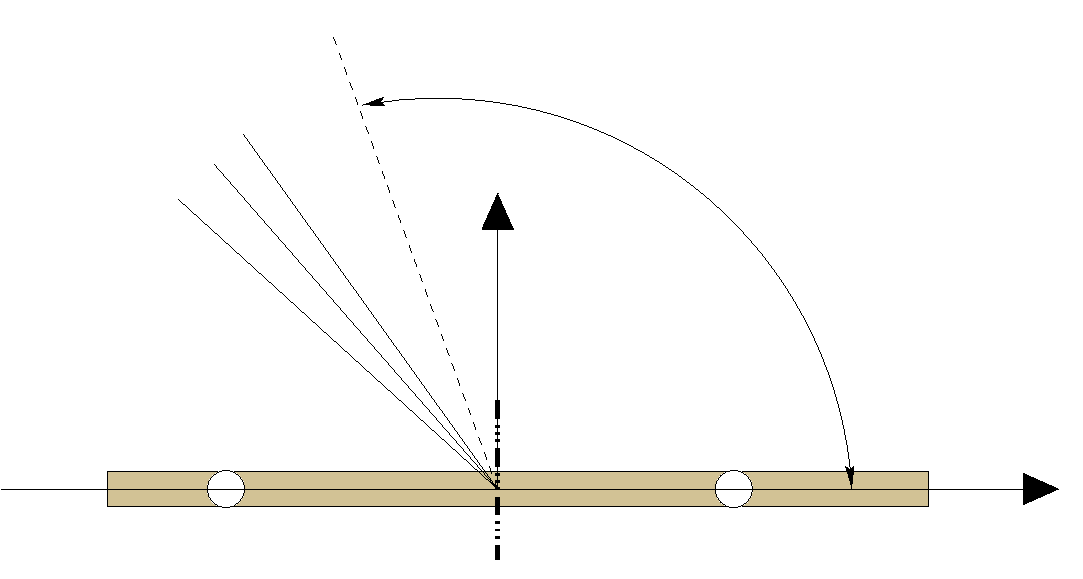
\includegraphics[width=0.5\textwidth]{\mainpath/fig/png/riemann}
        \caption[Riemann problem setup]{Solution of the 1D half Riemann problem around edge $i-j$ described in equation \eqref{eq:half_riemann_problem}. The obtained fluid state at the interface is then used to evaluate the flux function, see equations~\eqref{eq:half_riemann_problem_original} and \eqref{eq:flux_with_reconstructed_value_fiver1}}
		\label{fig:riemann_sketch}
    \end{center}
\end{figure}

\begin{align}\label{eq:flux_with_reconstructed_value_fiver1}
\fluxesnum_{ij}=\fluxesnum_{ij}(\fstateprim_{ij},\fstateprim^{\star}_b, \normal_{ij})
\end{align}



\subsection{Second order \ac{FIVER}}\label{sec:fiver-2}
The original version of \ac{FIVER} has been outlined in chapter~\ref{sec:fiver-1}. This algorithm has been successfully applied to the solution of multi-phase flows, underwater implosion problems and fluid structure interaction. However, like most \ac{IBM} it suffers one distinct disadvantage: global convergence drops to first order with an $\order{1}$ error at the interface. This observation motivated the generalization of FIVER to second order global accuracy performed in \cite{Main2014}.\\


Here, we first extrapolate the fluid state at node $i$ to the real intersection point with the interface (see Figure~\ref{fig:FIVER_interchapter}).
\begin{align}
\dfstate_{\Gamma} = \dfstate_i + \nabla \dfstate_i(\dmpos_{\Gamma}-\dmpos_i)
\end{align}
The one-dimensional half-Riemann problem is solved at the material interface $\Gamma$
\begin{align}
\dfstateprim^{\star}_{\Gamma} = \dfstateprim^{\star}(\dfstateprim_\Gamma,\fluidvel_{wall},\normal_{wall})
\end{align}
Once this solution has been obtained inter-/extrapolate the fluid state back to the surrogate interface yielding $\dfstateprim^{\star}_{ij}$
\begin{align}
\dfstateprim^{\star}_{ij} = \dfstateprim^{\star}_{ij}(\dfstate^{\star}_\Gamma,\dfstate_i) 
\end{align}
The numerical flux can then be evaluated the usual way using the obtained fluid state value:
\begin{align}
\dresidual^c_{ij} = \dresidual^c_{ij}(\dfstate_{ij},\dfstate^{\star}_{ij}, \normal_{ij})
\end{align}
It has been proven in \cite{Main2014} that this approach recovers second order convergence in the vicinity of the interface and thus a second order global convergence can be achieved.


\section{Evaluation of the viscous terms at the interface}\label{sec:fiver_viscous_term}
Section \ref{sec:fiver_setup} dealt with the general setup of an embedded simulation, chapter~\ref{sec:fiver-1} introduced the first order version of \ac{FIVER} for the inviscid term, which was then generalized to second order in chapter~\ref{sec:fiver-2}. So far, the interested reader might have noticed that the ghost nodes depicted in figure~\ref{fig:FIVER_interchapter} have not yet been used. This is due to the \ac{FV} treatment of the inviscid term and the formulation of half Riemann problems to the surrogate interface. The viscous terms, however, is treated differently.\\
We have shown and explained thoroughly the \ac{FE} like evaluation of the viscous term \eqref{eq:nse_final_discretized}  in chapter \ref{sec:mixed_FV_FE_formulation}.


If one wants to keep the \ac{FE}-like evaluation of the viscous term,~\eqref{eq:nse_final_discretized} can be splitted as
\begin{align}\label{eq:fiver_viscous_split}
\sum_{T_i \in \elementset(i)} \int_{T_i} \difftensor \nabla \fstate \nabla \phi_i dx=
\sum_{T_i \in \left(\elementset(i^a)\right)} \int_{T_i} \difftensor \nabla \fstate \nabla \phi_i dx+
\sum_{T_i \in \left(\elementset(i)\setminus\elementset(i^a)\right)} \int_{T_i} \difftensor \nabla \fstate^R \nabla \phi_i dx=
\end{align}

where $\elementset(i^a)$ is the set of triangles that can be build from the active nodes around node $i$ and $\elementset(i)\setminus\elementset(i^a)$ are all the triangles where at least one node is inactive(ghost).\\
\\
The only difficulty now becomes the evaluation of the last term, meaning the integration over intersected elements, where at least on node is inactive, and thus does not have a fluid state solution.\\
We did not have that problem for the inviscid term of equation \eqref{eq:nse_final_discretized}, since a \ac{FV} approximation was chosen, and therefore we could construct a flux at the interface thanks to the half Riemann problem. No inactive node had to be considered.\\
For the viscous part, however, we want to keep the \ac{FE} like formulations described in \ref{sec:mixed_FV_FE_formulation} to avoid re-writing large portions of the code. If a triangle is cut by the interface, one or two nodes will therefore be labeled inactive, and be denoted as ghost-nodes.
Clearly, the fluid state vector at this ghost nodes is not defined. The question thus becomes how to evaluate this terms (last part in equation~\eqref{eq:fiver_viscous_split} ).\\
\\
The approach we take, that is also outlined in \cite{Farhat2014} is to reconstruct a pseudo fluid-state at the ghost points, such that the boundary conditions at the wall are fulfilled.

\subsection{Reconstruction of the fluid-state at ghost-nodes}\label{sec:ghost_node_reconstruction}

To explain the reconstruction at the ghost nodes, it again helps to consider Figure~\ref{fig:FIVER_interchapter}.\\
We also notice that the viscous flux, as defined in Equation \ref{eq:fluxes_diff}, only depends on the fluid velocity and the temperature.
Reconstruction of the velocity at the ghost node is straight forward. Assuming a linear interpolation inside the elements, the velocity at node $i$ is reconstructed such, that the stick condition is fulfilled at the interface.\\
As far as the reconstruction of the temperature is concerned, two different cases have to be considered: adiabatic walls and isothermal walls.\\
For an adiabatic wall, the temperature gradient at the wall is zero, which can be achieved by setting the temperature of the ghost note equal to that of node $i$. An isothermal wall boundary condition enforces a certain, constant temperature at the wall. Similar to the velocity boundary condition, this can be achieved by finding an appropriate ghost point value such that the condition is enforced.\\


\begin{figure}[h!]
	\begin{center}
        \includegraphics[width=0.8\textwidth]{\mainpath/fig/tikz/build/ghost_population}
        \caption[Ghost Point population]{Illustration of the ghost point population process. States at nodes $i,j,k$ are known from computation. States at mid-edges $kg$, $ig$ and $jg$ are the states we want to impose at the interface. The pressure and density are constantly extrapolated from the fluid states, whereas the velocity is set to the structure  velocity at the interface, A linear extrapolation is then performed form the active states over the stated at the intersections points to obtain the interpolated ghost states. Since the interpolated ghost state values are typically ambiguous, due to multiple edges connecting to one ghost node, a least-square algorithm or a simple averaging can be performed to obtain a final value for the ghost state $\fstate_g$.}
		\label{fig:ghost_population}
    \end{center}
\end{figure}


The issue is depicted in detail in figure~\ref{fig:ghost_population}.
The figure also reveals that there is no unique solution for the ghost point value. Multiple active node connect to the ghost node and the above described relations can be formulated for every one of them. \ac{FIVER} therefore solves a least square system to chose an appropriate value.\\
The elegance of this approach is that once the ghost points states have been found, the evaluation of the viscous contribution can be done with the standard code routines. No adaption is required to make them work in the embedded framework.


\section{Evaluation of forces}\label{sec:fiver_force_evaluation}
Another issue that arises for embedded simulations is the appropriate evaluation of the forces on an embedded interface. This is especially important if the embedded framework is used in an \ac{FSI} setup to get an appropriate resultant on the structure.\\
Sensitivity Analysis is another application, where appropriate evaluation of Lift and Drag integrals are crucial.\\
This problem has been analyzed in \cite{Wang2011}\cite{Wang2012}.\\
Most importantly, the question becomes whether to evaluate the pressure integral~\eqref{eq:lift_and_drag_integrals} over the auxiliary control volume interface (figure~\ref{fig:FIVER_interchapter}) or over the so called reconstructed interface, which can be obtained by creating auxiliary surfaces inside the intersected elements through the knowledge of intersection points at the edges. Detailed information about the intersection detection is provided in\cite{Wang2011a}



\section{The level-set method}\label{sec:interface_tracking}

The issue of interface tracking is extensively discussed in \cite{Wang2012} and \cite{Fedkiw2003}.\\

Since the interface in an embedded stimulation typically moves, an appropriate interface tracking approach is required.\\
For \ac{FIVER}, the popular level set method \cite{Sethian1999} was chosen.

The level set approach is characterized by the following equation:
\begin{align}\label{eq:level_set}
\pdfrac{\phi}{t}+\fluidvel\cdot\nabla\phi=0 \Leftrightarrow \pdfrac{\phi}{t}+\nabla\cdot(\fluidvel\phi)=-\phi\nabla\cdot\fluidvel
\end{align}

where $\phi$ is a function designed to track the material interface. Particularly, $\phi$ is initialized such that that the interface is characterized by $\phi=0$. The interface can then be tracked via a simple discretization and time integration of equation~\eqref{eq:level_set}.
A periodic reinitialization of $\phi$ is sometimes necessary in order to maintain an optimal level of numerical accuracy.\\ 
Details of this approach, which was developed for computer visualization purposes, can be found in \cite{Sethian1999}.


\end{document}
